\documentclass{beamer}
%\usepackage[utf8]{inputenc}
%\usetheme{Warsaw}
\usetheme{CambridgeUS}
%\usecolortheme{seahorse}

%-------------------------------------------------------------------------------
%          -Packages nécessaires pour écrire en Français et en UTF8-
%-------------------------------------------------------------------------------
\usepackage[utf8]{inputenc}
\usepackage[frenchb]{babel}
\usepackage[T1]{fontenc}
\usepackage{lmodern}
\usepackage{textcomp}

%-------------------------------------------------------------------------------

%-------------------------------------------------------------------------------
%                          -Outils de mise en forme-
%-------------------------------------------------------------------------------
\usepackage{hyperref}
\hypersetup{pdfstartview=XYZ}
\usepackage{enumerate}
\usepackage{graphicx}
%\usepackage{multicol}
%\usepackage{tabularx}

%\usepackage{anysize} %%pour pouvoir mettre les marges qu'on veut
%\marginsize{2.5cm}{2.5cm}{2.5cm}{2.5cm}

\usepackage{indentfirst} %%pour que les premier paragraphes soient aussi indentés
\usepackage{verbatim}
%\usepackage[table]{xcolor}  
%\usepackage{multirow}
\usepackage{ulem}
%-------------------------------------------------------------------------------


%-------------------------------------------------------------------------------
%                  -Nécessaires pour écrire des mathématiques-
%-------------------------------------------------------------------------------
\usepackage{amsfonts}
\usepackage{amssymb}
\usepackage{amsmath}
\usepackage{amsthm}
\usepackage{tikz}
\usepackage{xlop}
\usepackage[output-decimal-marker={,}]{siunitx}
%-------------------------------------------------------------------------------


%-------------------------------------------------------------------------------
%                    - Mise en forme 
%-------------------------------------------------------------------------------

\newcommand{\bu}[1]{\underline{\textbf{#1}}}


\usepackage{ifthen}


\newcommand{\ifTrue}[2]{\ifthenelse{\equal{#1}{true}}{#2}{$\qquad \qquad$}}

\newcommand{\kword}[1]{\textcolor{red}{\underline{#1}}}


%-------------------------------------------------------------------------------



%-------------------------------------------------------------------------------
%                    - Racourcis d'écriture -
%-------------------------------------------------------------------------------

% Angles orientés (couples de vecteurs)
\newcommand{\aopp}[2]{(\vec{#1}, \vec{#2})} %Les deuc vecteurs sont positifs
\newcommand{\aopn}[2]{(\vec{#1}, -\vec{#2})} %Le second vecteur est négatif
\newcommand{\aonp}[2]{(-\vec{#1}, \vec{#2})} %Le premier vecteur est négatif
\newcommand{\aonn}[2]{(-\vec{#1}, -\vec{#2})} %Les deux vecteurs sont négatifs

%Ensembles mathématiques
\newcommand{\naturels}{\mathbb{N}} %Nombres naturels
\newcommand{\relatifs}{\mathbb{Z}} %Nombres relatifs
\newcommand{\rationnels}{\mathbb{Q}} %Nombres rationnels
\newcommand{\reels}{\mathbb{R}} %Nombres réels
\newcommand{\complexes}{\mathbb{C}} %Nombres complexes


%Intégration des parenthèses aux cosinus
\newcommand{\cosP}[1]{\cos\left(#1\right)}
\newcommand{\sinP}[1]{\sin\left(#1\right)}

%Fractions
\newcommand{\myfrac}[2]{{\LARGE $\frac{#1}{#2}$}}

%Vocabulaire courrant
\newcommand{\cad}{c'est-à-dire}

%Droites
\newcommand{\dte}[1]{droite $(#1)$}
\newcommand{\fig}[1]{figure $#1$}
\newcommand{\sym}{symétrique}
\newcommand{\syms}{symétriques}
\newcommand{\asym}{axe de symétrie}
\newcommand{\asyms}{axes de symétrie}
\newcommand{\seg}[1]{$[#1]$}
\newcommand{\monAngle}[1]{$\widehat{#1}$}
\newcommand{\bissec}{bissectrice}
\newcommand{\mediat}{médiatrice}
\newcommand{\ddte}[1]{$[#1)$}

%Figures
\newcommand{\para}{parallélogramme}
\newcommand{\paras}{parallélogrammes}
\newcommand{\myquad}{quadrilatère}
\newcommand{\myquads}{quadrilatères}
\newcommand{\co}{côtés opposés}
\newcommand{\diag}{diagonale}
\newcommand{\diags}{diagonales}
\newcommand{\supp}{supplémentaires}
\newcommand{\car}{carré}
\newcommand{\cars}{carrés}
\newcommand{\rect}{rectangle}
\newcommand{\rects}{rectangles}
\newcommand{\los}{losange}
\newcommand{\loss}{losanges}


%----------------------------------------------------

\title{Parallélogrammes particuliers}
\author{}\institute{}


\AtBeginSubsection[]
{
	\begin{frame}
		\frametitle{}
		\tableofcontents[currentsection, currentsubsection]
	\end{frame} 
}

\begin{document}
	
	
	
\begin{frame}
	\titlepage
\end{frame}

\section{Rappels sur les parallélogrammes}

\subsection{Définition}

\begin{frame}
\frametitle{ }  
\framesubtitle{ }	

\begin{columns}[onlytextwidth]
	\begin{column}{0.465\textwidth}
		\begin{exampleblock}{Définition}
			Un \textbf{\underline{\para\ }} est un \myquad\ dont les \underline{côtés opposés sont parallèles}.
		\end{exampleblock}	
		
		\begin{alertblock}{Propriété}
			Un \para\ admet un centre de symétrie: le \underline{point d'intersection des \diags\ }
		\end{alertblock}		
	\end{column}
	\begin{column}{0.465\textwidth}
		\center{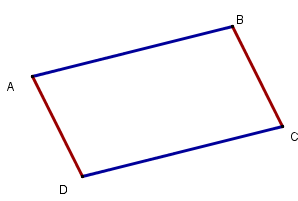
\includegraphics[scale=0.55]{./img/para}}
	\end{column}
\end{columns}


\end{frame}


\subsection{Propriétés}

\begin{frame}
	\frametitle{}  
	\framesubtitle{}	
	
	\begin{alertblock}{Propriété des \diags\ }
		Si un \myquad\ est un \para , alors ses \diags\ se coupent en leur milieu (\cad , elles ont le même milieu).
	\end{alertblock}
	
	\begin{alertblock}{Propriétés des côtés}<2->
		\begin{itemize}
			\item Si un \myquad\ est un \para , alors ses \underline{\co\ sont parallèles.}
			\item Si un \myquad\ est un \para , alors ses \underline{\co\ sont de même longueur}.
		\end{itemize}
	\end{alertblock}
	
\end{frame}




\begin{frame}
	\frametitle{}  
	\framesubtitle{}

	\begin{alertblock}{Propriétés des angles}
		\begin{itemize}
			\item Si un \myquad\ est un \para , alors ses \underline{angles opposés sont de même mesure.}
			\item Si un \myquad\ est un \para , alors \underline{2 angles consécutifs sont \supp}.
		\end{itemize}
	\end{alertblock}
		
	
	
\end{frame}



\section{Parallélogrammes particuliers}

\begin{frame}
	\frametitle{}
	\tableofcontents[currentsection, currentsubsection]
\end{frame} 

\begin{frame}
	\frametitle{}  
	\framesubtitle{}	
	
	\begin{alertblock}{Propriété (admise)}
		Le \rect , le \los , et le \car\ sont des \paras\ particuliers.
	\end{alertblock}
	
\end{frame}

\subsection{Le rectangle}

\begin{frame}
	\frametitle{}  
	\framesubtitle{}

\begin{columns}[onlytextwidth]	
	\begin{column}{0.7\textwidth}
		\begin{exampleblock}{Définition}
			Un \rect\ est un \myquad\ qui a quatre angles droits.
		\end{exampleblock}
		
		\begin{block}{Remarque}
			Un rectangle possède toutes les propriétés du \para .
		\end{block}
		
	\end{column}
	\begin{column}{0.3\textwidth}
		\center{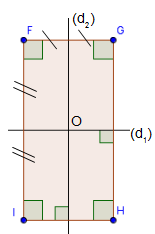
\includegraphics[scale=0.7]{./img/rect1}}
	\end{column}	
\end{columns}
\end{frame}

\begin{frame}
	\frametitle{}  
	\framesubtitle{}
	
	\begin{columns}[onlytextwidth]	
		\begin{column}{0.7\textwidth}

		\begin{alertblock}{Propriété (admise)}
			Un \rect\ possède deux axes de \sym\ : les médiatrices de ses côtés. (Il possède aussi un centre de \sym\ à l'intersection de ses \diags , comme tout \para)
		\end{alertblock}
		
		\begin{block}{Exemple}
			$(d_1)$ et $(d_2)$ sont les axes de \sym\ du \rect\ $FGHI$
		\end{block}
	\end{column}
	\begin{column}{0.3\textwidth}
		\center{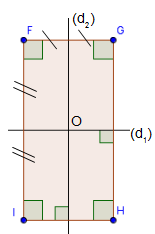
\includegraphics[scale=0.7]{./img/rect1}}
	\end{column}	
\end{columns}
	
\end{frame}


\begin{frame}
	\frametitle{}  
	\framesubtitle{}
	
		
	\begin{columns}[onlytextwidth]	
		
		\begin{column}{0.4\textwidth}
			\center{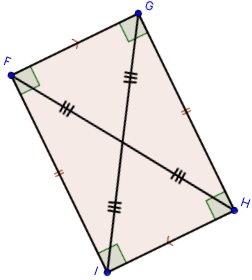
\includegraphics[scale=0.85]{./img/rect2}}
		\end{column}
		
		\begin{column}{0.6\textwidth}
			
			\begin{alertblock}{Propriété (admise)}
				Les \diags\ d'un \rect\ sont de même longueur.
			\end{alertblock}
			
			\begin{alertblock}{Prouver qu'un quadrilatère est un rectangle}
				\begin{itemize}
					\item Un \myquad\ a trois angles droits.
					\item Un \para\ possède un angle droit.
					\item Un \para\ possède des \diags\ de même longueur.
					\item Un \myquad\ a ses \diags\ qui se coupent en leur milieu et de même longueur.
				\end{itemize}
			\end{alertblock}
			
		\end{column}
		
	\end{columns}
	
\end{frame}
\subsection{Le losange}

\begin{frame}
	\frametitle{}  
	\framesubtitle{}
	
	\begin{columns}[onlytextwidth]	
		\begin{column}{0.65\textwidth}
			\begin{exampleblock}{Définition}
				Un \los\ est un \myquad\ qui a quatre côtés de même longueur.
			\end{exampleblock}
			
			\begin{block}{Remarque}
				Un rectangle possède toutes les propriétés du \para .
			\end{block}
			
		\end{column}
		\begin{column}{0.35\textwidth}
			\center{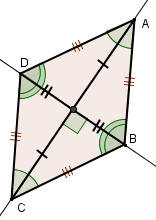
\includegraphics[scale=0.65]{./img/los}}
		\end{column}	
	\end{columns}
\end{frame}

\begin{frame}
	\frametitle{}  
	\framesubtitle{}
	
	\begin{columns}[onlytextwidth]	
		\begin{column}{0.65\textwidth}
			\begin{alertblock}{Propriétés (admises)}
				\begin{itemize}
					\item Un \los\ possède deux axes de \sym\ : ses \diags .
					(Comme tout parallélogramme, il possède aussi un centre de \sym\ à l'intersection de ses \diags .)
					
					\item Les \diags\ d'un \los\ sont perpendiculaires.
				\end{itemize}
				
			\end{alertblock}		
			
		\end{column}
		\begin{column}{0.35\textwidth}
			\center{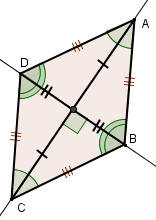
\includegraphics[scale=0.65]{./img/los}}
		\end{column}	
	\end{columns}
\end{frame}

\begin{frame}
	\frametitle{}  
	\framesubtitle{}
	
			
			\begin{alertblock}{Prouver qu'un \myquad\ est un losange}
				\begin{itemize}
					\item Un \myquad\ qui a ses quatre côtés de même longueur.
					\item Un \para\  qui possède deux côtés consécutifs de même longueur.
					\item Un \para\ qui a ses \diags\ perpendiculaires.
					\item Un \myquad\ qui a ses diagonales qui se coupent perpendiculairement en leur milieu.
				\end{itemize}
			\end{alertblock}
			
\end{frame}

\subsection{Le carré}

\begin{frame}
	\frametitle{}  
	\framesubtitle{}
	
	\begin{columns}[onlytextwidth]	
		\begin{column}{0.65\textwidth}
			\begin{exampleblock}{Définition}
				Un \car\ est un \myquad\ qui a quatre côtés de même longueur et quatre angles droits.
			\end{exampleblock}
			
			\begin{alertblock}{Propriété (admise)}
				Un \car\ est à la fois un \rect\ et un \los , donc il possède \textbf{toutes les propriétés du rectangle ET du losange}.
			\end{alertblock}
			
			\begin{alertblock}{Propriété (admise)}
				Un \car\ possède quatre axes de \sym\ : ses \diags\ et les \mediat s de ses côtés. (Comme tout parallélogramme, il possède aussi un centre de \sym\ à l'intersection de ses \diags .)
			\end{alertblock}
			
		\end{column}
		\begin{column}{0.35\textwidth}
			\center{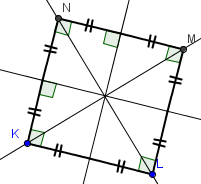
\includegraphics[scale=0.65]{./img/car1}}
		\end{column}	
	\end{columns}
\end{frame}


\begin{frame}
	\frametitle{}  
	\framesubtitle{}
	
	\begin{columns}[onlytextwidth]	
		\begin{column}{0.65\textwidth}
			
			\begin{alertblock}{Propriété }
				Les \diags\ d'un \car\ :
				\begin{itemize}
					\item[$\rightarrow$] ont la même longueur
					\item[$\rightarrow$] se coupent en leur milieu
					\item[$\rightarrow$] sont perpendiculaires
				\end{itemize}
			\end{alertblock}
			
			\begin{alertblock}{Prouver qu'un \myquad\ est un \car }
				On prouve que c'est un \los\ ET un \rect .
			\end{alertblock}
			
		\end{column}
		\begin{column}{0.35\textwidth}
			\center{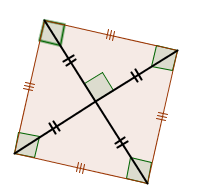
\includegraphics[scale=0.65]{./img/car2}}
		\end{column}	
	\end{columns}
\end{frame}

\section{Synthèse}

\begin{frame}
	\frametitle{}
	\tableofcontents[currentsection, currentsubsection]
\end{frame}

\begin{frame}
	\frametitle{}  
	\framesubtitle{}	
	
	\center{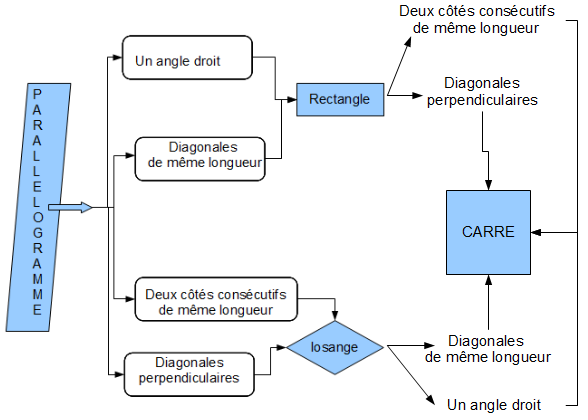
\includegraphics[scale=0.55]{./img/synthese}}
\end{frame}

\end{document}


\begin{frame}
	\frametitle{}  
	\framesubtitle{}	
	
\end{frame}